\chapter{Python-Übungen zu Kryptologie}\label{ch:Kryptologie}

\section{Allgemeine Zeichenketten-Aufgaben}
Zeichenketten können verkettet, also aneinandergehängt werden mit dem Befehl \lstinline|"Text1" + "Text2" + "Text3"| usw. Falls Sie eine Zeichenkette mehrfach drucken wollen, können Sie diese mit einer Zahl multiplizieren, die dann die Anzahl Wiederholungen der Zeichenkette bestimmt. So ist der Ausdruck \lstinline|"a" * 3| beispielsweise gleichbedeutend mit einer Zeichenkette \lstinline|"aaa"|.

Im Nachfolgenden schauen wir uns einige Übungen an, mit denen wir die einzelnen Zeichen aus Zeichenketten herauslesen können.

\begin{myexercise}
	Führen Sie das nachfolgende Programm aus und erklären Sie, was das Programm tut.
	\begin{lstlisting}
    text = "EASY"
    for buchstabe in text:
      print(buchstabe)
  \end{lstlisting}
	\begin{myanswer}
		\begin{lstlisting}
      E
      A
      S
      Y
    \end{lstlisting}
		\lstinline|for x in mystring| ist eine Schleife über die Zeichenkette \lstinline|mystring|. Dabei nimmt \lstinline|x| nacheinander jeden Buchstaben in dieser Zeichenkette genau einmal an.
	\end{myanswer}
\end{myexercise}

\begin{myexercise}\label{myexercise:index}
	Führen Sie das nachfolgende Programm aus und erklären Sie, was das Programm tut.
	\begin{lstlisting}
    Klartext = "Schweiz"
    print(Klartext[0])
    print(Klartext[1])
    print(Klartext[2])
    print(Klartext[3])
    print(Klartext[4])
    print(Klartext[5])
    print(Klartext[6])
  \end{lstlisting}
	\begin{myanswer}
		\begin{lstlisting}
      S
      c
      h
      w
      e
      i
      z
    \end{lstlisting}
		\lstinline|mystring[0]| ist der erste Buchstabe der Zeichenkette \lstinline|mystring|, \lstinline|mystring[1]| der zweite und so weiter.
	\end{myanswer}
\end{myexercise}

\begin{myexercise}
	Führen Sie das nachfolgende Programm aus und erklären Sie, was das Programm tut.
	\begin{lstlisting}
    Klartext = "Schweiz"
    for i in range(len(Klartext)):
      print(Klartext[i])
  \end{lstlisting}
	\begin{myanswer}
		Dieses Programm ist äquivalent zum Programm in \cref{myexercise:index}.
		Hier wird allerdings eine \lstinline|for|-Schleife über die Länge des Texts verwendet.
	\end{myanswer}
\end{myexercise}

Der Befehl \lstinline|for i in range(len(Klartext))| erstellt eine Variable \lstinline|i| innerhalb der \lstinline|for|-Schleife, welche jedes Zeichen von 0 bis zur Länge von \lstinline|Klartext| minus 1 geht. Weshalb minus 1? Das erste Zeichen von \lstinline|Klartext| wird in Python mit \lstinline|Klartext[0]| ausgelesen, das letzte mit \lstinline|Klartext[len(Klartext)-1]|, da wir bei 0 zu zählen beginnen und nicht bei 1. Mit dem Ausdruck \lstinline|Klartext[i]| wird also das \lstinline|i|-te Zeichen der Zeichenkette \lstinline|Klartext| ausgelesen, wobei \lstinline|i| von 0 bis zu (Länge des Klartexts minus 1) geht.

Der Befehl \lstinline|for i in range(len(Klartext))| kann auch geschrieben werden als Befehl \lstinline|for i in range(0, len(Klartext), 1)|, wobei dies meint:
\begin{itemize}
	\item \lstinline|i| beginnt bei 0
	\item \lstinline|i| geht bis zu \lstinline|len(Klartext)-1|
	\item \lstinline|i| vergrössert sich in 1er-Schritten
\end{itemize}
Dieser Befehl könnte auch verwendet werden, um bei einer beliebigen Zahl zu starten (nicht notwendigerweise 0), und um \lstinline|i| in Schritten grösser als 1 zu vergrössern. Die allgemeine Syntax des Befehls lässt sich also wie folgt zusammenfassen: \lstinline|for i in range(start, ende, schrittgroesse)|.

\begin{mychallenge}
    Eine Person verrät uns lediglich die Vorwahl ihrer $10$-stelligen Mobiltelefonnummer. Zudem verrät sie Ihnen auch, dass ihre Telefonnummer gerade ist (also auf 2, 4, 6, 8 oder 0 endet).
	Damit gibt es nur noch $5$ Millionen Kombinationen, die es (im schlimmsten Fall) auszuprobieren gilt.
	Schreiben Sie ein Python-Programm, welches die $200$ kleinsten, geraden Nummern auflistet.
	Die erste Nummer sollte $0790000000$ sein, die letzte $0790000198$.
	Das Programm soll die Nummern als Zeichenkette (eine Nummer pro Zeile) ausgeben.

	Tipps:
	\begin{itemize}
		\item Mit \lstinline|str(num)|
		      wird aus der Zahl \lstinline|num| eine Zeichenkette.
		      Beispielsweise gibt uns \lstinline|str(15)|
		      die Zeichenkette \lstinline[language=Python,basicstyle=\ttfamily\normalsize]!"15"!.
		\item Erinnern Sie sich, was die Operation \lstinline|+| in dem Ausdruck \lstinline[language=Python,basicstyle=\ttfamily\normalsize]!"In" + "form" + "atik"! macht?
	\end{itemize}
	\begin{myanswer}
		\begin{lstlisting}
      for num in range(790000000, 790000200,2):
        print("0" + str(num)) # füge die Zeichenkette "0" vorne an
    \end{lstlisting}
	\end{myanswer}
\end{mychallenge}


\section{Verschlüsselung von Texten in Python}
Während des Zweiten Weltkriegs arbeitete der brillante Mathematiker Alan Turing in Bletchley Park im Vereinten Königreich und war mit der entscheidenden Aufgabe betraut, den Enigma-Code zu knacken, den die Deutschen zur Verschlüsselung ihrer Nachrichten verwendeten. Um diesen komplexen Code zu entschlüsseln, musste Turing sein tiefes Verständnis von Sprache und Mustern nutzen. In diesem Kapitel folgen wir in Turings Fussstapfen und entziffern einige Geheimnachrichten!

\begin{figure}[H]
\centering
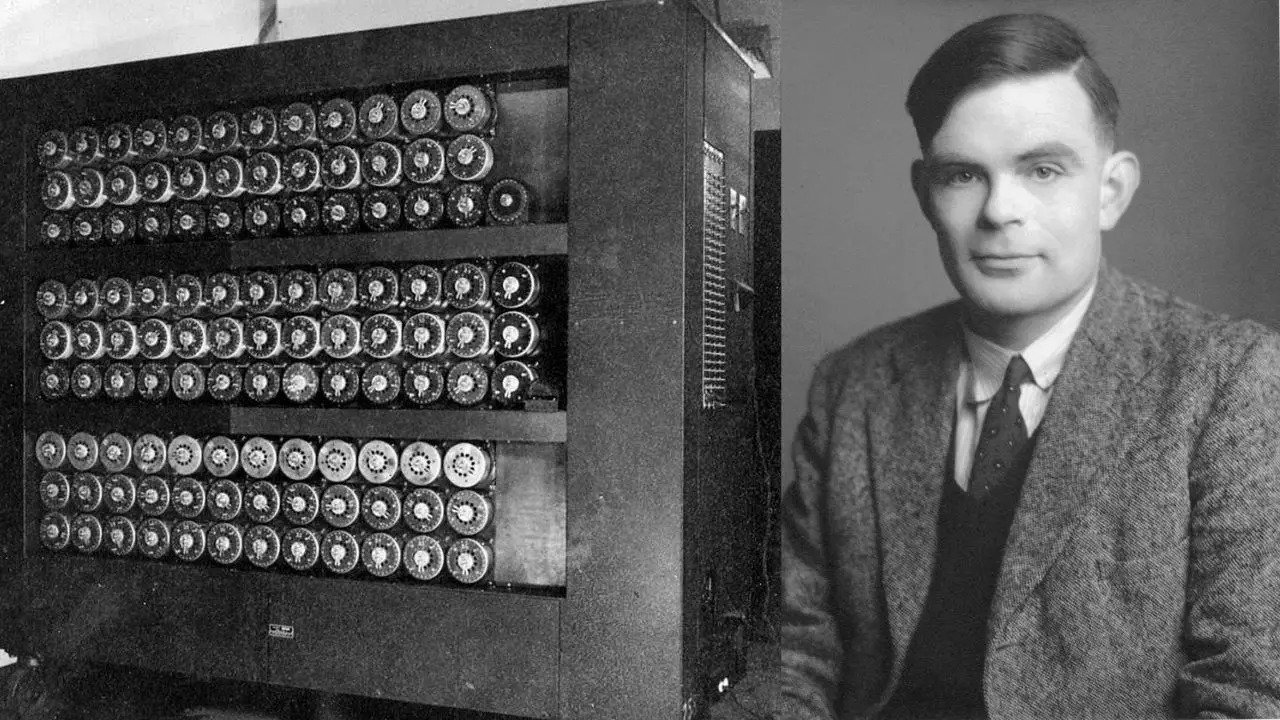
\includegraphics[width=0.7\linewidth]{Grundlagen_Info/03_Kryptologie/Figures/turing}
\caption{Turing mit seiner berühmten Turing-Maschine}
\label{fig:turing}
\end{figure}

Im Nachfolgenden schauen wir uns einige Python-Befehle an, die dazu dienen, mit Zeichenketten (= engl. \textit{strings}) zu arbeiten. Dies werden wir insbesondere benötigen, um eigene Python-Programme zu schreiben, mit denen wir Texte verschlüsseln und entschlüsseln können. Genauer gesagt bezeichnen wir Texte in Python als Zeichenketten. Zeichenketten werden in Python innerhalb von einfachen oder doppelten Anführungszeichen geschrieben, also entweder \lstinline|'...'| oder \lstinline|"..."|. Innerhalb der Anführungszeichen können beliebige Zeichen stehen, beispielsweise Buchstaben, Leerzeichen, Spezialzeichen oder Zahlen.


\cref{tab:string-op} und \cref{tab:string-sep-merge} enthalten eine Übersicht einiger nützlicher Befehle, die Sie in diesem Kapitel verwenden werden.

\begin{table}[H]
 \centering
\begin{tabular}{l|p{0.3\linewidth}|p{0.4\linewidth}}
\textbf{Python} & \textbf{Beschreibung} & \textbf{Beispiel} \\\midrule\midrule
\lstinline|len(s)| & Gibt die Länge des Textes \lstinline|s| zurück. & 

\begin{minipage}{\linewidth}
\begin{lstlisting}[numbers=none]
n = len("hallo") # 5
\end{lstlisting}
\end{minipage} \\\midrule\midrule
\lstinline|s[index]| & Greift auf das Zeichen an der Index-Position \lstinline|index| zu. Bei negativen Indizes zählt man von rechts. & \begin{minipage}{\linewidth}
\begin{lstlisting}[numbers=none]
s = "hallo"
c0 = s[0]  # "h"
c1 = s[1]  # "a"
c2 = s[-1] # "o"
\end{lstlisting}
\end{minipage}
 \\\midrule
\lstinline|s[start:end]| & Extrahiert den Teiltext vom Index \lstinline|start| bis und ohne \lstinline|end| & \begin{minipage}{\linewidth}
\begin{lstlisting}[numbers=none]
s1 = "hallo"
s2 = s1[1:4] # "all"
\end{lstlisting}
\end{minipage}\\\midrule\midrule
\lstinline|ord(c)| & Gibt die Position des Zeichens \lstinline|c| in der \href{https://en.wikipedia.org/wiki/List_of_Unicode_characters}{Unicode-Tabelle} zurück & \begin{minipage}{\linewidth}
\begin{lstlisting}[numbers=none]
n1 = ord('A') # 65
n2 = ord('B') # 66
n3 = ord('Z') # 90
\end{lstlisting}
\end{minipage}\\\midrule
\lstinline|chr(n)| & Gibt das Zeichen an der \lstinline|n|-ten Position der \href{https://en.wikipedia.org/wiki/List_of_Unicode_characters}{Unicode-Tabelle} zurück & \begin{minipage}{\linewidth}
\begin{lstlisting}[numbers=none]
c1 = chr(65) # "A"
c2 = chr(66) # "B"
c3 = chr(67) # "C"
\end{lstlisting}\end{minipage}\\\midrule\midrule
\lstinline|s1.count(s2)| & Zählt, wie oft der Text \lstinline|s2| im Text \lstinline|s1| vorkommt & \begin{minipage}{\linewidth}
\begin{lstlisting}[numbers=none]
s1 = "Das Haus ist gross und das Dach ist grün."
s2 = "ist"
n = s1.count(s2) # 2
\end{lstlisting}
\end{minipage}\\\midrule
\lstinline|s1.find(s2)| & Gibt den niedrigsten Index des Teiltexts \lstinline|s2| zurück, falls dieser vorhanden ist, ansonsten \lstinline|-1| & \begin{minipage}{\linewidth}
\begin{lstlisting}[numbers=none]
s = "Das Haus ist gross und das Dach ist grün."
n = s.find("ist") # 9
\end{lstlisting}
\end{minipage}\\\midrule
\lstinline|s1.replace(old, new)| & Ersetzt alle Vorkommen des Teil-Texts \lstinline|old| durch \lstinline|new|. & \begin{minipage}{\linewidth}
\begin{lstlisting}[numbers=none]
s1 = "hallo"
s2 = s1.replace("a", "e") # "hello"
\end{lstlisting}
\end{minipage}
\end{tabular}
\caption{Übersicht von Zeichenketten-Befehlen}
\label{tab:string-op}
\end{table}
\begin{myexercise}
Schreiben Sie ein Programm, um jeden Buchstaben \enquote{e / E} des folgenden Texts durch den Buchstaben \enquote{a / A} zu ersetzen:

\begin{lstlisting}
my_text = "Eines Tages entschied der Elefant, einen edlen Teppich zu weben."
\end{lstlisting}

\begin{myanswer}
\begin{lstlisting}
my_text = "Eines Tages entschied der Elefant, einen edlen Teppich zu weben."
my_text = my_text.replace("e", "a")
my_text = my_text.replace("E", "A")
print(my_text)
\end{lstlisting}
\end{myanswer}
\end{myexercise}

\begin{myexercise}
Schreiben Sie ein Programm, um zu zählen, wie häufig der Buchstabe \enquote{e / E} im gesamten folgenden Text vorkommt:

\begin{lstlisting}
my_text = "Eines Tages entschied der Elefant, einen edlen Teppich zu weben."
\end{lstlisting}

\begin{myanswer}
\begin{lstlisting}
my_text = "Eines Tages entschied der Elefant, einen edlen Teppich zu weben."
n_e = my_text.count("e")
n_e += my_text.count("E")
print(n_e) # 15
\end{lstlisting}
\end{myanswer}
\end{myexercise}


\begin{mychallenge}
Was könnte der Nutzen davon sein, dass es zwei Möglichkeiten gibt und nicht nur eine, Zeichenketten zu schreiben (\lstinline|'...'| oder \lstinline|"..."|)?
\begin{myanswer}
Eine Möglichkeit, die uns durch die unterschiedlichen Schreibweisen geboten wird, ist, Anführungszeichen auszugeben. Beispielsweise könnten Sie so einen Text, der Anführungszeichen beinhaltet, auf der Konsole drucken:
\begin{lstlisting}
print('Meine Freunde nennen mich "Mr. X"')
\end{lstlisting}
\end{myanswer}
\end{mychallenge}

Mit der \textbf{Länge} von Zeichenketten ist die Anzahl der Zeichen zwischen den Anführungszeichen gemeint: Die Zeichenkette \lstinline|"Hello World"| hat beispielsweise eine Länge von 11 Zeichen. Die Länge einer Zeichenkette kann mit dem Ausdruck \lstinline|len(Klartext)| bestimmt werden.

\begin{myexercise}
	Bestimmen Sie die Länge Ihres vollen Namens mithilfe des Befehls \lstinline|len()| in Python.
\begin{lstlisting}[numbers=none]
n = "Vorname Nachname"
print(len(n)) # 16
\end{lstlisting}
\end{myexercise}

Die Lösung für \cref{ex:zweiertausch} könnte in Python wie folgt implementiert werden:
\lstinputlisting{Grundlagen_Info/03_Kryptologie/Python package/encryption/zweiertausch.py}

 \begin{myexercise}
 Schreiben Sie eine Python-Funktion \lstinline|def dreiertausch(klartext)|, welche den \enquote{Dreiertausch} aus der Einführungsaufgabe 2 implementiert.
 \begin{myanswer}
\lstinputlisting{Grundlagen_Info/03_Kryptologie/Python package/encryption/dreiertausch.py}
 \end{myanswer}
 \end{myexercise}
 
  \begin{myexercise}
  Schreiben Sie eine Python-Funktion \lstinline|def umkehren(klartext)|, welche alle Zeichen eines Klartexts in umgekehrter Reihenfolge ausgibt.
  \begin{myanswer}
\lstinputlisting{Grundlagen_Info/03_Kryptologie/Python package/encryption/umkehren.py}
  \end{myanswer}
  \end{myexercise}
  
 \newpage
 

 \begin{table}[H]
 \centering
 \begin{tabular}{l|p{0.3\linewidth}|p{0.4\linewidth}}
 \textbf{Python} & \textbf{Beschreibung} & \textbf{Beispiel} \\\midrule\midrule
 
 \lstinline|s1.split(sep)| & Zerlegt den Text an jedem \texttt{sep} und gibt eine Liste der Teiltexte zurück.  & \begin{minipage}{\linewidth}
 \begin{lstlisting}[numbers=none]
s = "a,b,c"
li = s.split(",") 
# ["a", "b", "c"]
\end{lstlisting}
 \end{minipage}\\\midrule
  \lstinline|s.join(li)| & Verbindet die Elemente von \texttt{li} zu einem Text, getrennt durch den Text \texttt{s}.  & \begin{minipage}{\linewidth}
  \begin{lstlisting}[numbers=none]
txt = ":".join(["a", "b", "c"]) 
# "a:b:c"
\end{lstlisting}
  \end{minipage}\\\midrule
   \lstinline|str(n)| & Zahl \texttt{n} in einen Text (engl. \textit{string}) umwandeln  & \begin{minipage}{\linewidth}
   \begin{lstlisting}[numbers=none]
 n = 10
 s = str(n) # "10"
\end{lstlisting}
   \end{minipage}\\\midrule
    \lstinline|int(s)| & Text \texttt{s} in eine ganze Zahl (engl. \textit{integer}) umwandeln  & \begin{minipage}{\linewidth}
    \begin{lstlisting}[numbers=none]
s = "10"
n = int(s) # 10
\end{lstlisting}
    \end{minipage}
 \end{tabular}
 \caption{Übersicht von Befehlen, um Zeichenketten zu verbinden, bzw. trennen}
 \label{tab:string-sep-merge}
 \end{table}
 \begin{myexercise}
Der Schlüssel für einen Geheimtext ist in Blöcken organisiert:

\begin{lstlisting}
geheime_zahl_als_text = "2_10_38"
\end{lstlisting}

Trennen Sie die Blöcke von \lstinline|geheime_zahl_als_text| in eine Liste auf und addieren Sie die Zahlen der Liste zusammen.

Als Resultat sollten Sie die Zahl 50 erhalten.
\begin{myanswer}
\begin{lstlisting}
geheime_zahl_als_text = "2_10_38"
meine_liste = geheime_zahl_als_text.split("_")
summe = 0
for i in meine_liste:
    summe += int(i)
    
print(summe)
\end{lstlisting}
\end{myanswer}
 \end{myexercise}
 
 \begin{myexercise}
Verbinden Sie die Wörter in der Liste \lstinline|liste = ["Der", "Code", "wurde", "geknackt"]| mit Leerzeichen zu einem vollständigen Satz.
\begin{myanswer}
\begin{lstlisting}
liste = ["Der", "Code", "wurde", "geknackt"]
print(" ".join(liste))
\end{lstlisting}
\end{myanswer}
 \end{myexercise}

\newpage
\section{Caesar-Verschlüsselung in Python}
\begin{myexercise}\label{ex:oneline}
Entwickeln Sie eine Funktion, die zwei Parameter entgegennimmt: den Klartext (nur Grossbuchstaben!) und den Schlüssel (0-25). Als erstes soll jeder Buchstaben des Klartexts auf einer neuen Zeile ausgegeben werden. 

Beispiel: Falls der Text \texttt{HALLO} eingegeben wird, soll folgendes ausgegeben werden:
\begin{lstlisting}[language=bash]
H
A
L
L
O
\end{lstlisting}
\begin{myanswer}
\begin{lstlisting}
def verschluessle(klartext, schluessel):
    for buchstabe in klartext:
        print(buchstabe)

verschluessle("HALLO", 3)
\end{lstlisting}
\end{myanswer}
\end{myexercise}

\begin{myexercise}\label{ex:oneline-ascii}
Passen Sie das Programm aus \cref{ex:oneline} so an, dass statt den Buchstaben die Position in der Unicode-Tabelle ausgegeben wird. Verwenden Sie dafür die Funktion \lstinline|ord()|.

Beispiel: Falls der Text \texttt{HALLO} eingegeben wird, soll folgendes ausgegeben werden:
\begin{lstlisting}[language=bash]
72
65
76
76
79
\end{lstlisting}
\begin{myanswer}
\begin{lstlisting}
def verschluessle(klartext, schluessel):
    for buchstabe in klartext:
        print(ord(buchstabe))

verschluessle("HALLO", 3)
\end{lstlisting}
\end{myanswer}
\end{myexercise}

\begin{myexercise}\label{ex:oneline-ascii-shift}
Passen Sie das Programm aus \cref{ex:oneline-ascii} so an, dass Sie zu den Unicode-Positionen auch noch die Verschiebung hinzurechnen. 

Beispiel: Falls der Text \texttt{HALLO} eingegeben wird und die Verschiebung 2, soll folgendes ausgegeben werden:
\begin{lstlisting}[language=bash]
74
67
78
78
81
\end{lstlisting}
\begin{myanswer}
\begin{lstlisting}
def verschluessle(klartext, schluessel):
    for buchstabe in klartext:
        print(ord(buchstabe) + schluessel)

verschluessle("HALLO", 2)
\end{lstlisting}
\end{myanswer}
\end{myexercise}

\begin{myexercise}\label{ex:oneline-ascii-shift-char}
Passen Sie das Programm aus \cref{ex:oneline-ascii-shift} so an, dass Sie statt den verschobenen Unicode-Positionen die Buchstaben ausgeben. Verwenden Sie dafür die Funktion \lstinline|chr()|.
 

Beispiel: Falls der Text \texttt{HALLO} eingegeben wird und die Verschiebung 2, soll folgendes ausgegeben werden:
\begin{lstlisting}[language=bash]
J
C
N
N
Q
\end{lstlisting}
\begin{myanswer}
\begin{lstlisting}
def verschluessle(klartext, schluessel):
    for buchstabe in klartext:
        print(chr(ord(buchstabe) + schluessel))

verschluessle("HALLO", 2)
\end{lstlisting}
\end{myanswer}
\end{myexercise}

\begin{myexercise}\label{ex:oneline-ascii-shift-char-safety}
Wenn man den Klartext \texttt{ZORRO} mit dem Schlüssel 14 verschlüsselt, erhält man mit dem Programm aus Aufgabe \cref{ex:oneline-ascii-shift-char} den Geheimtext \lstinline|h]``]|. Eigentlich sollte man aber den Geheimtext \texttt{NCFFC} erhalten. Lösen Sie das Problem!

Tipp: Der grösste gültige Unicode-Wert ist 90 für den Buchstaben \enquote{\texttt{Z}}. Wenn man einen Wert bekommt, der 91 oder grösser ist, muss man ihn verkleinern!

\begin{myanswer}
\begin{lstlisting}
def caesar(klartext, schluessel):
    for buchstabe in klartext:
        n = ord(buchstabe) + schluessel
        if n>90:
            n-=26
        print(chr(n))

caesar("ZORRO", 14)
\end{lstlisting}
\end{myanswer}


\end{myexercise}

\begin{myexercise}\label{ex:oneline-ascii-shift-char-safety-final}
Passen Sie das Programm aus \cref{ex:oneline-ascii-shift-char-safety} so an, dass die Geheimtextbuchstaben nicht untereinander, sondern auf derselben Zeile in die Ausgabe geschrieben werden.

Tipp: Mit dem Operator \texttt{+} lassen sich in Python Texte miteinander verbinden.

\begin{lstlisting}
text = ""
text += "Hello"
text += " Bob"
print(text) # Hello Bob
\end{lstlisting}

Die verschlüsselte Zeichenkette soll per \lstinline|return|-Befehl zurückgegeben werden.

\begin{myanswer}
\begin{lstlisting}
def caesar(klartext, schluessel):
    kryptotext = ""
    for buchstabe in klartext:
        n = ord(buchstabe) + schluessel
        if n>90:
            n-=26
        kryptotext += chr(n)
        
    return kryptotext

res = caesar("ZORRO", 14)
print(res)
\end{lstlisting}
\end{myanswer}
\end{myexercise}

\begin{myexercise}
Entwickeln Sie ein Programm, das über einen Parameter den Geheimtext und den Schlüssel entgegennimmt und dann mit Hilfe der Caesar-Chiffre den Klartext wiederherstellt. Testen Sie es anschliessend, indem Sie eine verschlüsselte Nachricht von Ihrer Sitznachbarin oder Ihrem Sitznachbar entschlüsseln!

\begin{myanswer}
\begin{lstlisting}
def caesar_ent(kryptotext, schluessel):
    klartext = ""
    for buchstabe in kryptotext:
        n = ord(buchstabe) - schluessel
        if n<65:
            n+=26
        klartext += chr(n)
        
    return klartext

res = caesar_ent("NCFFC", 14)
print(res)
\end{lstlisting}
\end{myanswer}
\end{myexercise}

\section{Vigenère-Verschlüsselung in Python}

\begin{myexercise}\label{ex:vig}
Entwickeln Sie eine Funktion \lstinline|def vigenere(text, key)|, die über die zwei Parameter \lstinline|text| und \lstinline|key| einen Klartext sowie einen Schlüssel entgegennimmt. Das Programm soll den Klartext mit der Vigenère-Chiffre und mit dem Schlüssel verschlüsseln.
\begin{myanswer}
\begin{lstlisting}
def vigenere(text, key, encrypt=True):
    text_encrypted = []
    for i in range(len(text)):
        if text[i] != " ":
            k = key[i % len(key)]
            shift = ord(k)-65
            if encrypt:
                new_letter = chr(((shift+ord(text[i])-65) % 26)+65)
            else:
                new_letter = chr(((ord(text[i])-65-shift) % 26)+65)
            text_encrypted.append(new_letter)
        else:
            text_encrypted.append(" ")

    text_encrypted = "".join(text_encrypted)
    return text_encrypted
    
print(vigenere("TESTTEXT", "KEY", encrypt=True))
\end{lstlisting}
\end{myanswer}
\end{myexercise}

\begin{myexercise}
Entwickeln Sie eine Funktion \lstinline|def vigenere_ent(text, key)|, die über die zwei Parameter \lstinline|text| und \lstinline|key| einen Geheimtext sowie einen Schlüssel entgegennimmt. Das Programm soll den Geheimtext mit der Vigenère-Chiffre und mit dem Schlüssel entschlüsseln.

\begin{myanswer}
Gleicher Code wie in \cref{ex:vig}, aber mit Parameter \lstinline|encrypt=False| beim Aufruf
\end{myanswer}
\end{myexercise}

\begin{mychallenge}
Sie wollen all ihre Passwörter auf einer lokalen Textdatei abspeichern. Dies ist jedoch nicht sicher, denn falls jemand ihren Computer knackt, kann die Person alle Passwörter einsehen. Sie kommen auf folgende Idee: Statt die Passwörter aufzuschreiben, speichern Sie eine mit Vigenère verschlüsselte Variante davon. So müssen Sie sich lediglich den Vigenère-Schlüssel im Kopf merken, nicht aber ihre Passwörter. Verwenden Sie Ihr Programm aus \cref{ex:vig}, um ein Programm zu schreiben, das sie zuerst mit \lstinline|input| nach einem Schlüssel und einem verschlüsselten Passwort fragt. Das Programm gibt Ihnen danach ihr Passwort im Klartext zurück.
\begin{myanswer}
\begin{lstlisting}
def vigenere(encrypt=False):
    text = input("Wie lautet das verschlüsselte Passwort?")
    key = input("Wie lautet der Schlüssel?")
    text_encrypted = []
    for i in range(len(text)):
        if text[i] != " ":
            k = key[i % len(key)]
            shift = ord(k)-65
            if encrypt:
                new_letter = chr(((shift+ord(text[i])-65) % 26)+65)
            else:
                new_letter = chr(((ord(text[i])-65-shift) % 26)+65)
            text_encrypted.append(new_letter)
        else:
            text_encrypted.append(" ")

    text_encrypted = "".join(text_encrypted)
    return text_encrypted
    
print(vigenere(encrypt=False))
\end{lstlisting}
\end{myanswer}
\end{mychallenge}

\begin{myexercise}[Häufigkeitsanalyse und Caesar]
Eine Nachricht wurde abgefangen: \lstinline|msg = "AZDIYDHRZNOZI"|.

\begin{itemize}
\item Die Nachricht wurde mit der Caesar-Chiffre verschlüsselt. Finden Sie  zunächst einmal den häufigsten Buchstaben in der verschlüsselten Nachricht. \textbf{Tipp}: \enquote{A} und \enquote{Z} haben die Positionen 65 und 90 im Unicode. Um in einer Schleife alle Zahlen von \texttt{x} by \texttt{y} durchzugehen, können Sie Folgendes schreiben: \lstinline|for num in range(x, y+1):|.

\item Bestimmen Sie den verwendeten Schlüssel, indem Sie die Funktion \lstinline|ord()| zweimal verwenden.

\item Ermitteln Sie den Klartext mithilfe Ihres Programms aus \cref{ex:oneline-ascii-shift-char-safety-final}. \textbf{Tipp}: Das häufigste Zeichen in einem deutschen Text ist in der Regel \enquote{E}.

\item Ersetzen Sie am Schluss im Klartext das Wort \enquote{WESTEN} durch \enquote{OSTEN}.

\end{itemize}
\begin{myanswer}
\begin{lstlisting}
txt = "AZDIYDHRZNOZI"
for num in range(65,91):
    print(chr(num), txt.count(chr(num)))
    
x = caesar_ent(txt, ord("Z")-ord("E"))
res = x.replace("WESTEN","OSTEN")
\end{lstlisting}
\end{myanswer}
\end{myexercise}

\begin{myexercise}
Gegeben sei die durchschnittliche Buchstabenhäufigkeit für alle Buchstaben des deutschen Alphabets. Diese lässt sich berechnen, indem man die Häufigkeiten für sehr lange deutsche Texte aufsummiert.

\begin{lstlisting}[numbers=none]
german_letter_frequencies = [6.51, 1.89, 3.06, 5.08, 17.40, 1.66, 3.01, 4.76, 7.55, 0.27, 1.21, 3.44, 2.53, 9.78, 2.51, 0.79, 0.02, 7.00, 7.27, 6.15, 4.35, 0.67, 1.89, 0.03, 0.04, 1.13]
\end{lstlisting}

Berechnen Sie mithilfe des folgenden Python-Programms die Friedmansche Charakteristik für diese Häufigkeiten.
\lstinputlisting[numbers=none]{Grundlagen_Info/03_Kryptologie/Python package/encryption/friedman.py}
\end{myexercise}


